\begin{tikzpicture}[
  ->, % makes the edges directed
  >=stealth', % makes the arrow heads bold
  node distance=3cm, % specifies the minimum distance between two nodes. Change if necessary.
  every state/.style={thick, fill=gray!10}, % sets the properties for each ’state’ node
  initial text=$ $, % sets the text that appears on the start arrow
]
\node[state, initial] (start) {$v_1$};
\node[state, right of=start] (pe) {$v_2$};
\node[state, right of=pe, accepting] (pes-filipes) {$v_3$};
\node[state, below of=pes-filipes, accepting] (pejsek) {$v_4$};
\node[state, below of=pejsek, accepting] (maxipes-fik) {$v_5$};

\node[right of=pes-filipes] (pes-filipes-drawing) {\scalebox{-1}[1]{
\includegraphics[height=2cm,trim={0 4.75cm 0 0},clip]{figures/pes-filipes}}};
\node[right of=pejsek] (pejsek-drawing) {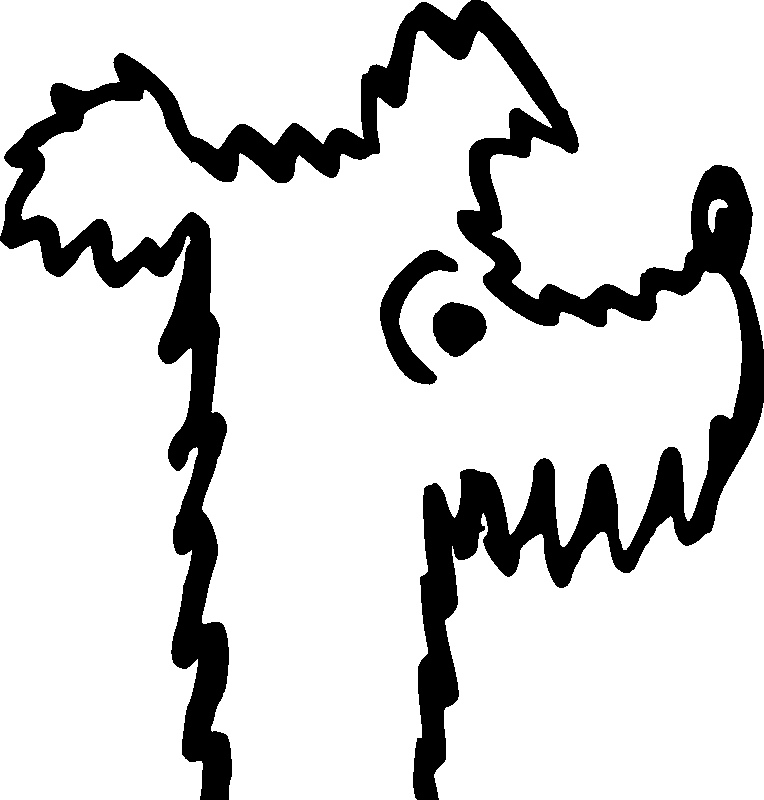
\includegraphics[height=2cm]{figures/pejsek}};
\node[right of=maxipes-fik] (maxipes-fik-drawing) {
\includegraphics[height=2cm]{figures/maxipes-fik}};

\draw (start) edge node[above]{pe} (pe);
\draw (pe) edge node[above]{s\textvisiblespace filipes} (pes-filipes);
\draw (pes-filipes) edge (pes-filipes-drawing);
\draw (pe) edge node[above, rotate=-45]{jsek} (pejsek);
\draw (pejsek) edge (pejsek-drawing);
\draw (start) edge node[above, rotate=-45]{maxipes\textvisiblespace fík} (maxipes-fik);
\draw (maxipes-fik) edge (maxipes-fik-drawing);
\end{tikzpicture}